\documentclass[12pt,a4paper]{article}
\usepackage{fullpage}
\usepackage[top=2cm, bottom=4.5cm, left=2.5cm, right=2.5cm]{geometry}
\usepackage{amsmath,amsthm,amsfonts,amssymb,amscd}
\usepackage{lastpage}
\usepackage{enumerate}
\usepackage{fancyhdr}
\usepackage{mathrsfs}
\usepackage{xcolor}
\usepackage{wrapfig}
\usepackage{graphicx}
\usepackage{listings}
\usepackage{hyperref}
\usepackage{txfonts}
\usepackage{titlesec}
\usepackage{floatflt}
\usepackage{esint}

\hypersetup{%
  colorlinks=true,
  linkcolor=blue,
  linkbordercolor={0 0 1}
}


\newcommand\course{8.03x - Vibrations and Waves}
\newcommand\hwnumber{1}               
\newcommand\MyName{Syed Suhaib Ahmad}
 
\renewcommand\lstlistingname{Algorithm}
\renewcommand\lstlistlistingname{Algorithms}
\def\lstlistingautorefname{Alg.}

\setlength{\parindent}{0.0in}
\setlength{\parskip}{0.05in}



\pagestyle{fancyplain}
\headheight 35pt
\lhead{\course}
\chead{\large\textbf{Problem Set 2}}
\rhead{\MyName{}}
\lfoot{}
\cfoot{\small\thepage}
\rfoot{}
\headsep 1.5em

\begin{document}

\subsubsection*{Problem 2.1 - Driven oscillator with damping}
An object of mass 0.2\,kg is hung from a spring whose spring constant is 80\,N/m. The body is subject to a resistive force given by $-bv$, where $v$ is its velocity (m/sec) and $b=4\,\text{Nm}^{-1}$sec.
\begin{enumerate}
    \item[(a)]Set up the differential equation of motion for free oscillations of the system, and find the period of such oscillations.
    \item[(b)]The object is subjected to a sinusoidal force given by $F(t)=F_0\sin\omega t$, where $F_0=2$\,N and $\omega=30\,\text{sec}^{-1}$. In the steady state, what is the amplitude of the forced oscillation?
\end{enumerate}
Instead of a driving force (see (b)), we now oscillate the end of the spring at the top end vertically with a harmonic displacement $X=X_0\sin(\omega t)$.
\begin{enumerate}
    \item[(c)]Set up the differential equation of motion for this driven oscillator.
    \item[(d)]What is the amplitude of the mass in steady state for $\omega=0$, 30 and 300 sec$^{-1}$? $X_0=0.5$\,cm in all cases.
\end{enumerate}
\textbf{Solution(a)}
\\
\\There are two forces acting on the system, spring and resistive force, that cause a resultant force. Applying Newton's second law
\[F_{\text{net}}=-kx-bv\Rightarrow m\frac{d^2x}{dt^2}=-kx-b\frac{dx}{dt}\]
\begin{equation}
    \Rightarrow \frac{d^2x}{dt^2}+\gamma\frac{dx}{dt}+\omega_0^2x=0.
\end{equation}
Equation (1) shows a simple harmonic oscillation, where $\gamma=b/m=20\,\text{s}^{-1}$ and $\omega_0=\sqrt{k/m}=20\,\text{s}^{-1}$. Since $\omega_0>\gamma/2$, system is underdamped with a time period of
\[T=\frac{2\pi}{\omega}=\frac{2\pi}{\sqrt{\omega_0^2-\frac{\gamma^2}{4}}}\approx0.36\,\text{s}.\]
\textbf{Solution(b)}
\\
\\With the addition of this driving force, equation (1) now becomes
\begin{equation}
    \frac{d^2x}{dt^2}+\gamma\frac{dx}{dt}+\omega_0^2x=\frac{F_0}{m}\sin\omega t.
\end{equation}
This differential equation has a steady state solution of the form
\[x(t)=A\cos(\omega t-\delta)\]
where $\delta$ is the phase delay between the driver and mass, $\omega$ is the driving frequency and $A$ is the amplitude, which is given by
\begin{equation}
    A=\frac{F_0/m}{\sqrt{(\omega_0^2-\omega^2)^2+(\gamma\omega)^2}}.
\end{equation}
Substituting the given values into equation (3) gives the amplitude of the forced oscillations to be approximately 1.28\,cm.
\newpage
\textbf{Solution(c)}
\\
\\If the spring is extended by a positive displacement $X$ in the upward direction and consequently contracted by $x$ from the other end, the restoring force on the mass becomes
\[F_{\text{restoring}}=+k(X-x).\]
Considering all forces on the mass and applying Newton's second law, we obtain
\[F_{\text{net}}=F_{\text{restoring}}+F_{\text{resistive}}\Rightarrow ma=k(X-x)-bv\]
\[\Rightarrow m\frac{d^2x}{dt^2}=kX-kx-b\frac{dx}{dt}\Rightarrow m\frac{d^2x}{dt^2}+b\frac{dx}{dt}+kx=kX\]
\begin{equation}
    \Rightarrow\frac{d^2x}{dt^2}+\gamma\frac{dx}{dt}+\omega_0^2x=\frac{kX_0}{m}\sin\omega t.
\end{equation}
\textbf{Solution(d)}
\\
\\As equation (4) is almost identical as equation (3), the amplitude for this system in steady state is 
\begin{equation}
    A=\frac{kX_0/m}{\sqrt{(\omega_0^2-\omega^2)^2+(\gamma\omega)^2}}.
\end{equation}
By substituting the values given in problem, we find that
\[A=\begin{cases}
    5.0\,\text{cm}
    \\0.256\,\text{cm}
    \\0.00237\,\text{cm}
\end{cases}\]
for $\omega=$ 0, 30 and 300\,s$^{-1}$ respectively.

\subsubsection*{Problem 2.2 - Seismograph}
\begin{floatingfigure}[r]{0.25\textwidth}
\vspace{-1em} % Adjust this value to align with the paragraph
\centering
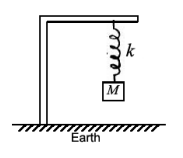
\includegraphics[width=0.2\textwidth]{figs/fig_prob_2.2.png}
\end{floatingfigure}
Imagine a simple seismograph consisting of a mass $M$ hung from a
spring on a rigid frame attached to the earth (see figure). The spring force and the damping force depend on the displacement and velocity relative to the earth’s surface, but the relevant acceleration (Newton’s 2nd law) of $M$ is relative to the fixed stars.
\vspace{0.4cm}
\begin{enumerate}
    \item[(a)]Using $y$ to denote the displacement of $M$ relative to the earth and $\eta$ to denote the displacement of the earth’s surface relative to the fixed stars, show that the equation of motion is
    \[\frac{d^2y}{dt^2}+\gamma\frac{dy}{dt}+\omega_0^2y=-\frac{d^2\eta}{dt}\]
    \item[(b)]Solve for $y$ (steady-state) if $\eta=C\cos\omega t$.
    \item[(c)]Sketch a graph of the amplitude $A$ of the displacement $y$ as a function of $\omega$ (supposing $C$ the same for all $\omega$).
    \item[(d)]A typical long-period seismometer has a period of about 30\,sec and a $Q$ of about 2. As the result of a violent earthquake the earth’s surface may oscillate with a period of about 20\,min and with an amplitude such that the maximum acceleration is about $10^{-9}$m/sec$^2$. How small a value of $A$ must be observable if this is to be detected?
    \item[(e)]Make sure you appreciate the big difference between this problem and problem 2.1. Compare the amplitudes of the two problems at very low and very high frequencies. 
\end{enumerate}
\par
\textbf{Solution(a)}
\\
\\Displacement between the mass and fixed stars is $s=y+\eta$ according to the given scenario. For an extension $y$ in the spring, there is a restoring force $-ky$ and similarly, there is a damping force $-bv$ on the mass $M$. Since the the acceleration of $M$ depends on the fixed stars, we use displacement $s$ for Newton's second law.
\[M\frac{d^2s}{dt^2}=-ky-b\frac{dy}{dt}\]
\[\frac{d^2}{dt^2}(y+\eta)=-\frac{k}{M}y-\frac{b}{M}\frac{dy}{dt}\]
\begin{equation}
    \frac{d^2y}{dt^2}+\gamma\frac{dy}{dt}+\omega_0^2y=-\frac{d^2\eta}{dt}.
\end{equation}
\textbf{Solution(b)}
\\
\\For $\eta=C\cos\omega t$, $\frac{d^2\eta}{dt^2}=-C\omega^2\cos\omega t$. Substituting $\frac{d^2\eta}{dt^2}$ into equation (6) gives
\begin{equation}
    \frac{d^2y}{dt^2}+\gamma\frac{dy}{dt}+\omega_0^2y=C\omega^2\cos\omega t.
\end{equation}
To solve this differential equation, we move to the complex plane and rewrite equation (7) as
\[\frac{d^2z}{dt^2}+\gamma\frac{dz}{dt}+\omega_0^2z=C\omega^2e^{j(\omega t)}\]
where
\[z=Ae^{j(\omega t-\delta)}.\]
Thus, the steady state solution of equation (7) must be $y=\text{Re}\,z$. The first and second derivatives of $z$ with respect to time are
\[\frac{dz}{dt}=Aj\omega e^{j(\omega t-\delta)}\,\,\,\,\,\text{and}\,\,\,\,\,\frac{d^2z}{dt^2}=-A\omega^2e^{j(\omega t-\delta)}.\]
Now, we have
\[e^{j(\omega t-\delta)}\left(-A\omega^2+Aj\omega\gamma+A\omega_0^2\right)=C\omega^2e^{j(\omega t)}\]
\[-A\omega^2+Aj\omega\gamma+A\omega_0^2=C\omega^2(\cos\delta+j\sin\delta).\]
Comparing coefficients,
\[A\left(\omega_0^2-\omega^2\right)=C\omega^2\cos\delta\,\,\,\,\,\text{and}\,\,\,\,\,A\omega\gamma=C\omega^2\sin\delta.\]
Solving these two equations simultaneously for $A$ and $\delta$ gives
\[\tan\delta=\frac{\omega\gamma}{\omega_0^2-\omega^2}\,\,\,\,\,\text{and}\,\,\,\,\,A=\frac{C\omega^2}{\sqrt{(\omega_0^2-\omega^2)^2+(\omega\gamma)^2}}.\]
Finally, the steady state solution to the differential equation in Eq. (7) is
\[y=\text{Re}\,z=A\cos(\omega t-\delta)\]
where $A$ is the amplitude and $\delta$ is the phase delay.
\\
\\\textbf{Solution(c)}
\\
\begin{figure}[h]
    \centering
    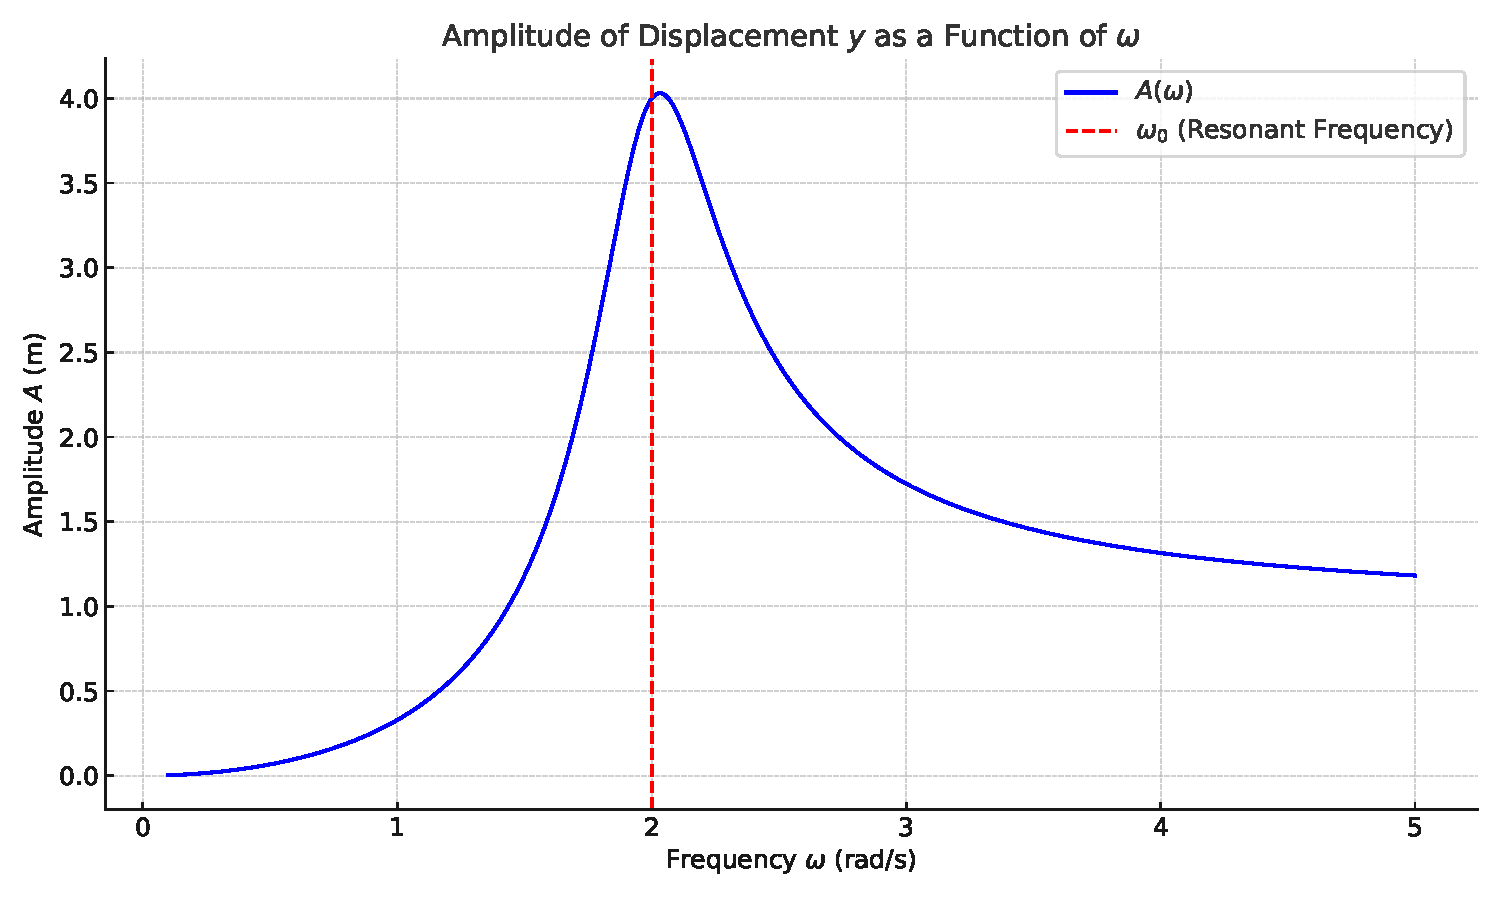
\includegraphics[width=1\linewidth]{figs/fig_sol_2.2c.pdf}
  %  \caption{Caption}
   % \label{fig:enter-label}
\end{figure}
\\\textbf{Solution(d)}
\\
\\Time period of seismometer is given by
\[T=\frac{2\pi}{\omega_0}\Rightarrow \omega_0=\frac{2\pi}{T}=\frac{2\pi}{30}=\frac{\pi}{15}\,\text{s}^{-1}.\]
\[Q=\frac{\omega_0}{\gamma}\Rightarrow\gamma=\frac{\omega_0}{Q}=\frac{\pi/15}{2}=\frac{\pi}{30}\,\text{s}^{-1}.\]
When the acceleration of earth's surface is maximum, $\omega t=0$, thus,
\[C\omega^2\cos0=a_{\text{max}}\Rightarrow C\omega^2=10^{-9}\,\text{ms}^{-2}.\]
Substituting all these values into the expression for amplitude of $y$.
\[A=\frac{10^{-9}}{\sqrt{((\pi/15)^2-(2\pi/(20\times60))^2)^2+(2\pi/(20\times60)\times\pi/30)^2}}=2.28\times10^{-8}\,\text{m}.\]
\textbf{Solution(e)}
\\
\\Calculating the amplitudes of both oscillations at extreme values gives some insight on how different these two systems are.
\begin{align*}
    &\omega=0:\,\,\,\,\,\,\,\,\,A_{2.1}=\frac{F_0}{m\omega_0^2}\,\,\,\,\,\,\,\,\,\,\,\,\,A_{2.2}=0
\\&\omega=\omega_0:\,\,\,\,\,A_{2.1}=\frac{F_0}{m\gamma\omega_0}\,\,\,\,\,\,\,\,\,\,A_{2.2}=QC
\\&\omega=\infty:\,\,\,\,\,\,A_{2.1}=0\,\,\,\,\,\,\,\,\,\,\,\,\,\,\,\,\,\,\,\,\,\,A_{2.2}=C.
\end{align*}
This shows, there is very significant difference between the oscillations as both behave differently for same values of $\omega$.

\subsubsection*{Problem 2.3 - Power dissipation}
The power input to maintain forced vibrations can be calculated by recognizing that this power is the mean rate of doing work against the resistive force $-bv$.
\begin{enumerate}
    \item[(a)]Satisfy yourself that the instantaneous rate of doing work against this force is equal to $bv^2$.
    \item[(b)]Using $x=A\cos(\omega t-\delta)$, show that the mean rate of doing work is $b\omega^2A^2/2$.
    \item[(c)]Substitute the value of $A$ at any arbitrary frequency and hence obtain the expression for $\Bar{P}$ as given in Eq. (4-23).
\end{enumerate}
\textbf{Solution(a)}
\\
\\We know that work done in moving an object a distance $dx$ against a force $F$ is given by the dot product of $-F$ and $dx$ and power is the rate of doing work. Using this information, we have
\[P=\frac{-\boldsymbol{\Vec{F}}\cdot d\boldsymbol{\Vec{x}}}{dt}=\frac{bv\,dx}{dt}=bv^2.\]
\textbf{Solution(b)}
\\
\\Differentiating $x$ with respect to time:
\[\frac{dx}{dt}=v=-A\omega\sin(\omega t-\delta).\]
For mean power, we use the average value of $\sin^2(\omega t-\delta)$, which $1/2$. Now,
\begin{equation}
    \Bar{P}=b(-A\omega)\times\frac{1}{2}=\frac{b\omega^2A^2}{2}.
\end{equation}
\textbf{Solution(c)}
\\
\\For this problem, we are going to use the following relationships
\[\omega_0^2=\frac{k}{m},\,\,\,\,\,\gamma=\frac{b}{m}\,\,\,\,\,\text{and}\,\,\,\,\,Q=\frac{\omega_0}{\gamma}.\]
The value of $A$ for a forced oscillation due to a harmonic force is given by equation (3). Putting this value into equation (8) gives
\[\Bar{P}=\frac{b\omega^2F^2_0}{2m^2\left(\left(\omega_0^2-\omega^2\right)^2+(\gamma\omega)^2\right)}=\frac{b\omega^2F_0^2}{2m^2\omega^2\omega_0^2\left(\left(\frac{\omega_0}{\omega}-\frac{\omega}{\omega_0}\right)^2+\left(\frac{\gamma}{\omega_0}\right)^2\right)}\]
\[=\frac{bF_0^2\omega_0}{2m\omega_0k\left(\left(\frac{\omega_0}{\omega}-\frac{\omega}{\omega_0}\right)^2+\left(\frac{\gamma}{\omega_0}\right)^2\right)}=\frac{F_0^2\omega_0\gamma}{2k\omega_0\left(\left(\frac{\omega_0}{\omega}-\frac{\omega}{\omega_0}\right)^2+\left(\frac{\gamma}{\omega_0}\right)^2\right)}\]
\begin{equation}
    \Bar{P}=\frac{F_0^2\omega_0}{2kQ\left(\left(\frac{\omega_0}{\omega}-\frac{\omega}{\omega_0}\right)^2+\frac{1}{Q^2}\right)}.
\end{equation}

\subsubsection*{Problem 2.4 - Transient behavior}
Consider the simple damped spring-mass system shown in the first figure. The mass is driven by an external force given by
\[F(t)=F_0\cos(\omega t+\phi)\]
The mass is at rest at its equilibrium position, $x=0$, when the force is turned on instantaneously
\begin{figure}[h]
    \centering
    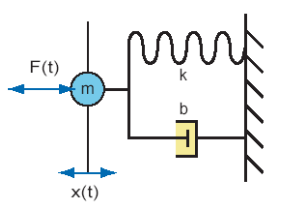
\includegraphics[width=0.4\linewidth]{figs/fig_prob_2.4.png}
  %  \caption{Caption}
 %   \label{fig:enter-label}
\end{figure}
at $t=0$. The response of the mass to this driving force in shown in the second figure. Assuming that the mass is $m=1$\,kg, use the time series for $x(t)$ to get estimates (within 20\%) for:
\begin{enumerate}
    \item[(a)]The natural frequency of the undamped oscillator, $\omega_0/(2\pi)$ in Hz.
    \\\textit{Hint: You may assume that $\gamma$ is small, so that $\omega_1\equiv\sqrt{\omega_0^2-\gamma^2/4}\approx\omega_0$.}
    \item[(b)]The damping coefficient, $b$ in N\,s/m.
    \item[(c)]The frequency of the driving force, $\omega/(2\pi)$ in Hz.
    \item[(d)]The amplitude of the driving force, $F_0$ in N.
    \item[(e)]What is $\phi$?
    \begin{figure}[h]
    \centering
    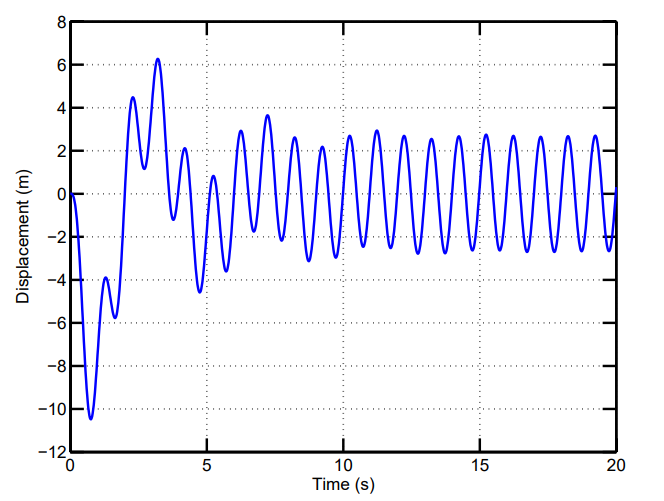
\includegraphics[width=0.7\linewidth]{figs/fig_prob_2.4e.png}
    %\caption{Caption}
   % \label{fig:enter-label}
\end{figure}
\end{enumerate}
\textbf{Solution(a)}
\\
\\From the graph, while the system is not in steady state, it can be seen that time period of one oscillation is approximately 4\,s.
\[\omega_0=\frac{2\pi}{T}=\frac{2\pi}{4}=\frac{\pi}{2}\,\text{rad\,s}^{-1}.\]
\textbf{Solution(b)}
\\
\\The factor responsible for damping is $e^{-\frac{\gamma}{2}t}$. Reading the graph at two points, $(-10.5,0.8)$ and $(6.2,3.2)$, gives
\[6.2=10.5e^{-\frac{\gamma}{2}(3.2-0.8)}\Rightarrow e^{1,2\gamma}=\frac{10.5}{6.2}\Rightarrow\gamma=\frac{\ln(10.5/6.2)}{1.2}\approx0.44\,\text{s}^{-1}.\]
We know that 
\[\gamma=\frac{b}{m}\Rightarrow b=m\gamma=1\times0.44=0.44\,\text{Nsm}^{-1}.\]
It is important to note that this value of $b$ is a very crude approximation.
\\
\\\textbf{Solution(c)}
\\
\\This part of the problem is relatively easier as graph clearly shows approximately five complete cycles, once the system settles to steady state, from $t=15$ to $t=20$\,s.
\[\omega=2\pi f\approx2\pi\times\frac{5}{5}\approx2\pi\,\text{rad\,s}^{-1}.\]
\textbf{Solution(d)}
\\
\\$F_0$ can be determined by manipulating equation (3).
\begin{equation}
    F_0=Am\sqrt{(\omega_0^2-\omega^2)^2+(\gamma\omega)^2}.
\end{equation}
Value of $A$, the amplitude of forced oscillations in steady state, can be directly read from the graph ($A\approx2.6\,$m). $\omega$ and $\omega_0$ have already been calculated in part (a) and (c) respectively. Equation (10) now becomes
\[F_0=2.6\sqrt{(\pi^2/4-4\pi^2)^2+(0.44\times2\pi)^2}\approx96\,\text{N}.\]
\textbf{Solution(e)}
\\
\\We assume that $\omega$ is greater enough than $\omega_0$ for $F(t)$ and $x(t)$ to be out of phase by $\pi$ radians. Also, upon extrapolating the steady state solution, we find that $x(t=0)=0$ and it starts in the positive direction. Thus, $F(t)$ must start in the negative direction and as the problem suggests, force is turned on instantaneously at $t=0$; $F(t=0)$ should also be zero. A rough plot of $F(t)$ and $x(t)$ is given below.
\begin{figure}[h!]
    \centering
    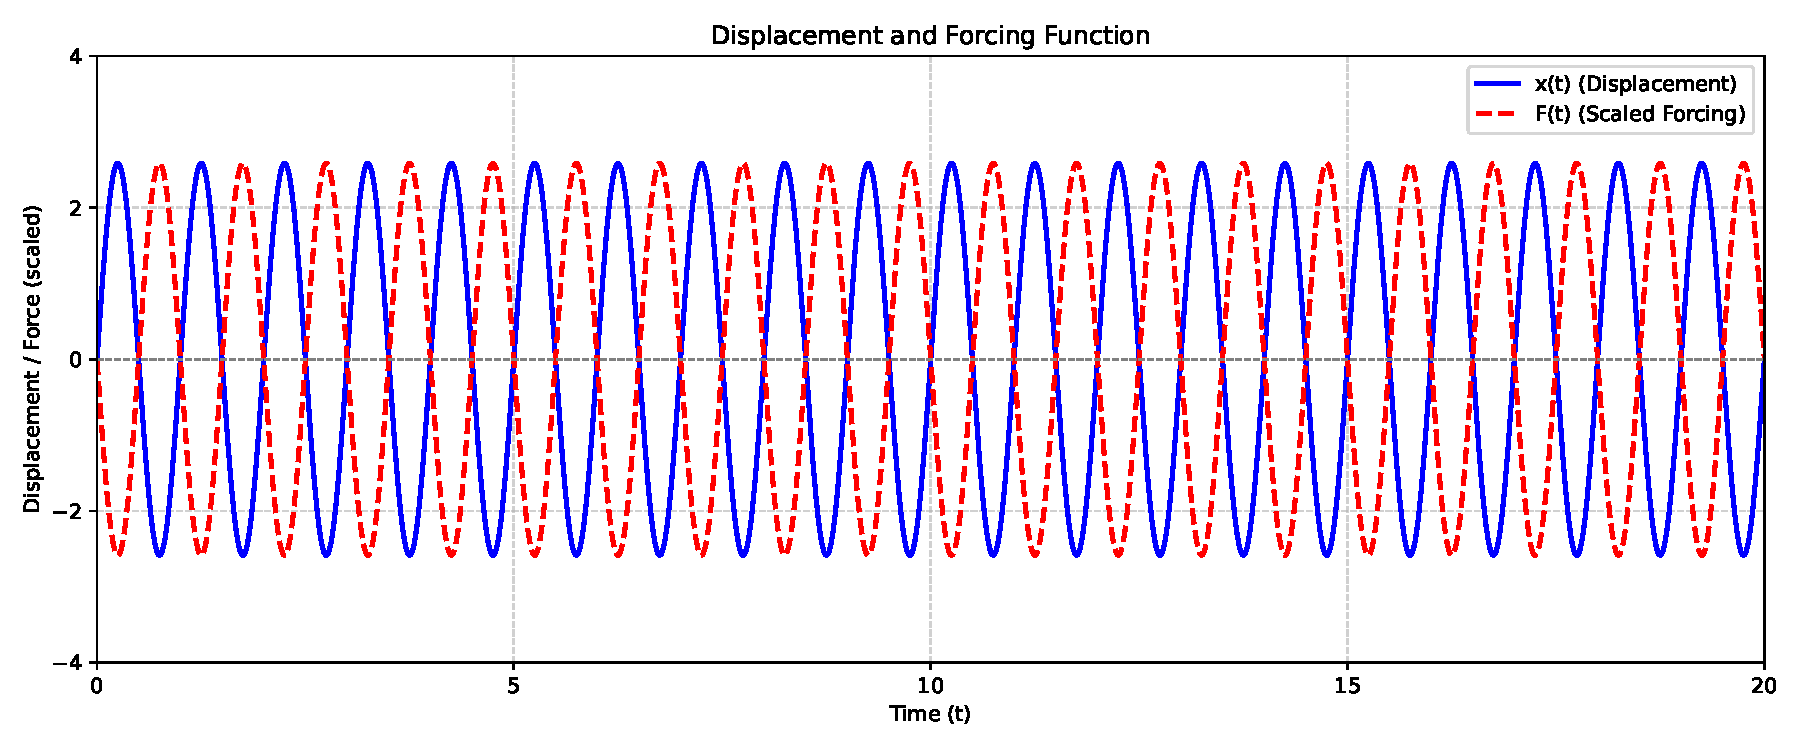
\includegraphics[width=1\linewidth]{figs/fig_sol_2.4e.pdf}
   % \caption{Caption}
  %  \label{fig:enter-label}
\end{figure}
\\Finally, we have
\[F(t=0)=F_0\cos\phi=0\Rightarrow\phi=\frac{\pi}{2}.\]
\subsubsection*{Problem 2.5 - Driven RLC circuit}
A generator of emf $V(t)=V_0\cos\omega t$ is connected in series with a resistance $R$, an inductance $L$, and a capacitance $C$.
\begin{enumerate}
    \item[(a)]Using Faraday’s law, write down the differential equations for the current $I$ in the circuit and for the charge, $q$, on the capacitor.
    \item[(b)]Solve for $q(\omega,t)$.
    \item[(c)]Solve for $I(\omega,t)$.
\end{enumerate}
In what follows, $V_0=3\,$V, $R=50\,\Omega$, $L=100$\,mH, and $C=0.01\,\mu$F.
\begin{enumerate}
    \item[(d)]Plot the amplitude of the current $(I_0)$ as a function of $\omega$.
    \item[(e)]At what value of $\omega$ is $(I_0)$ a maximum?
    \item[(f)]Plot $q_0$ as a function of $\omega$.
    \item[(g)]At what frequency, $\omega$, is the voltage across the capacitor a maximum?
\end{enumerate}
\textbf{Solution(a)}
\\
\\Potential difference across $R$, $L$ and $C$ is $V_R$, $V_L$ and $V_C$ respectively. Assume positive current flows in clockwise direction across the circuit. Applying Faraday's Law,
\begin{equation}
    \oint\boldsymbol{\Vec{E}}\cdot d\boldsymbol{\Vec{l}}=-\frac{d\Phi_B}{dt}
\end{equation}
(R.H.S of equation (11) can be written as $-L\frac{dI}{dt}$.)
\[V_R+V_L+V_C-V(t)=-L\frac{dI}{dt}\Rightarrow IR+0+\frac{q}{C}-V_0\cos\omega t=-L\frac{dI}{dt}\]
\[\Rightarrow R\frac{dq}{dt}+\frac{q}{C}+L\frac{d^2q}{dt^2}=V_0\cos\omega t\Rightarrow \frac{d^2q}{dt^2}+\frac{R}{L}\frac{dq}{dt}+\frac{q}{LC}=\frac{V_0}{L}\cos\omega t.\]
Given that
\[\frac{R}{L}=\gamma\,\,\,\,\,\text{and}\,\,\,\,\,\frac{1}{LC}=\omega_0^2.\]
Therefore, the differential equation found above now becomes
\begin{equation}
    \frac{d^2q}{dt^2}+\gamma\frac{dq}{dt}+\omega_0^2q=\frac{V_0}{L}\cos\omega t.
\end{equation}
Differentiating equation (12) once with respect to time gives a differential equation in terms of current $I$ in the circuit.
\begin{equation}
    \frac{d^2I}{dt^2}+\gamma\frac{dI}{dt}+\omega_0^2I=-\frac{V_0}{L}\omega\sin\omega t.
\end{equation}
\textbf{Solution(b)}
\\
\\As we have already solved a very similar kind of differential equation in problem 2.2, the solution to equation (12) follows the same analogy.
\[q(\omega,t)=q_0\cos(\omega t-\delta)\]
where
\[q_0=\frac{V_0/L}{\sqrt{\left(\omega_0^2-\omega^2\right)^2+(\gamma\omega)^2}}\,\,\,\,\,\text{and}\,\,\,\,\,\tan\delta=\frac{\gamma\omega}{\omega_0^2-\omega^2}.\]
\textbf{Solution(c)}
\\
\\An expression for current $I(\omega,t)$ can be directly determined by taking the time derivative of $q(\omega,t)$.
\[I(\omega,t)=\frac{dq(\omega,t)}{dt}=-q_0\omega\sin(\omega t-\delta)=-I_0\sin(\omega t-\delta)\]
where
\[I_0=\frac{\omega V_0/L}{\sqrt{\left(\omega_0^2-\omega^2\right)^2+(\gamma\omega)^2}}\,\,\,\,\,\text{and}\,\,\,\,\,\tan\delta=\frac{\gamma\omega}{\omega_0^2-\omega^2}.\]
\textbf{Solution(d)}
\begin{figure}[h]
    \centering
    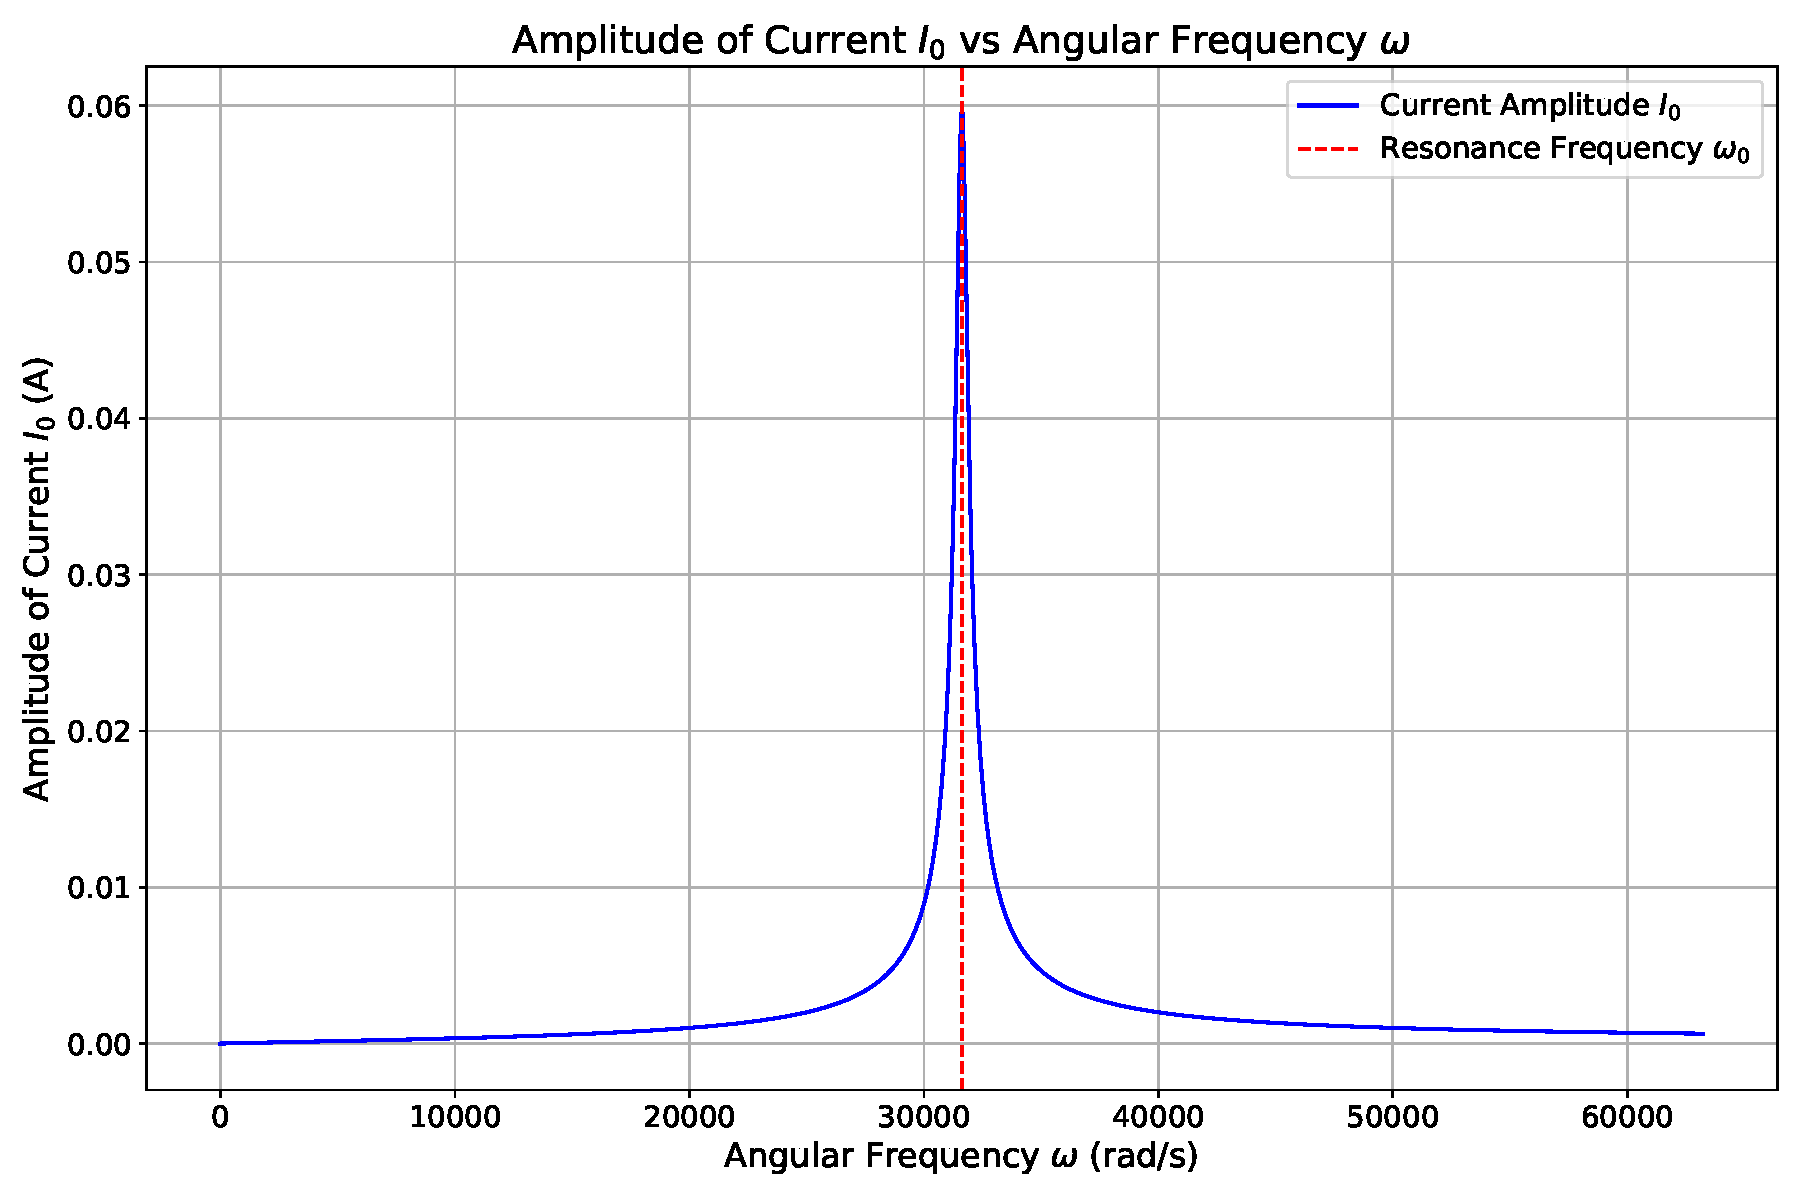
\includegraphics[width=1\linewidth]{figs/fig_sol_2.5d.pdf}
    %\caption{Caption}
   % \label{fig:enter-label}
\end{figure}
\\
\textbf{Solution(e)}
\\
\\If we rewrite the equation for $I_0$ by substituting back $\omega_0^2$ and $\gamma$, we get
\[I_0=\frac{\omega V_0/L}{\sqrt{\left(\frac{1}{(LC)^2}-\omega^2\right)^2+\left(\frac{R\omega}{L}\right)^2}}=\frac{\omega V_0/L}{\omega/L\sqrt{\left(\frac{1}{\omega C}-\omega L\right)^2+R^2}}\]
\begin{equation}
    I_0=\frac{V_0}{\sqrt{\left(\frac{1}{\omega C}-\omega L\right)^2+R^2}}.
\end{equation}
In equation (14), the terms $1/\omega C$ and $\omega L$ are known as capacitive and inductive reactances respectively ($X_C$ and $X_L$). They both have the units of resistance, that is, Ohms ($\Omega$). Thus, it is quite clear that $I_0$ is maximum when these two terms sort of “kill” each other. This leads to 
\[X_C=X_L\Rightarrow\frac{1}{\omega C}=\omega L\Rightarrow \omega=\frac{1}{\sqrt{LC}}=\frac{1}{\sqrt{0.1\times10^{-8}}}\approx3.162\times10^4\,\text{rad\,s}^{-1}.\]
\textbf{Solution(f)}
\begin{figure}[h]
    \centering
    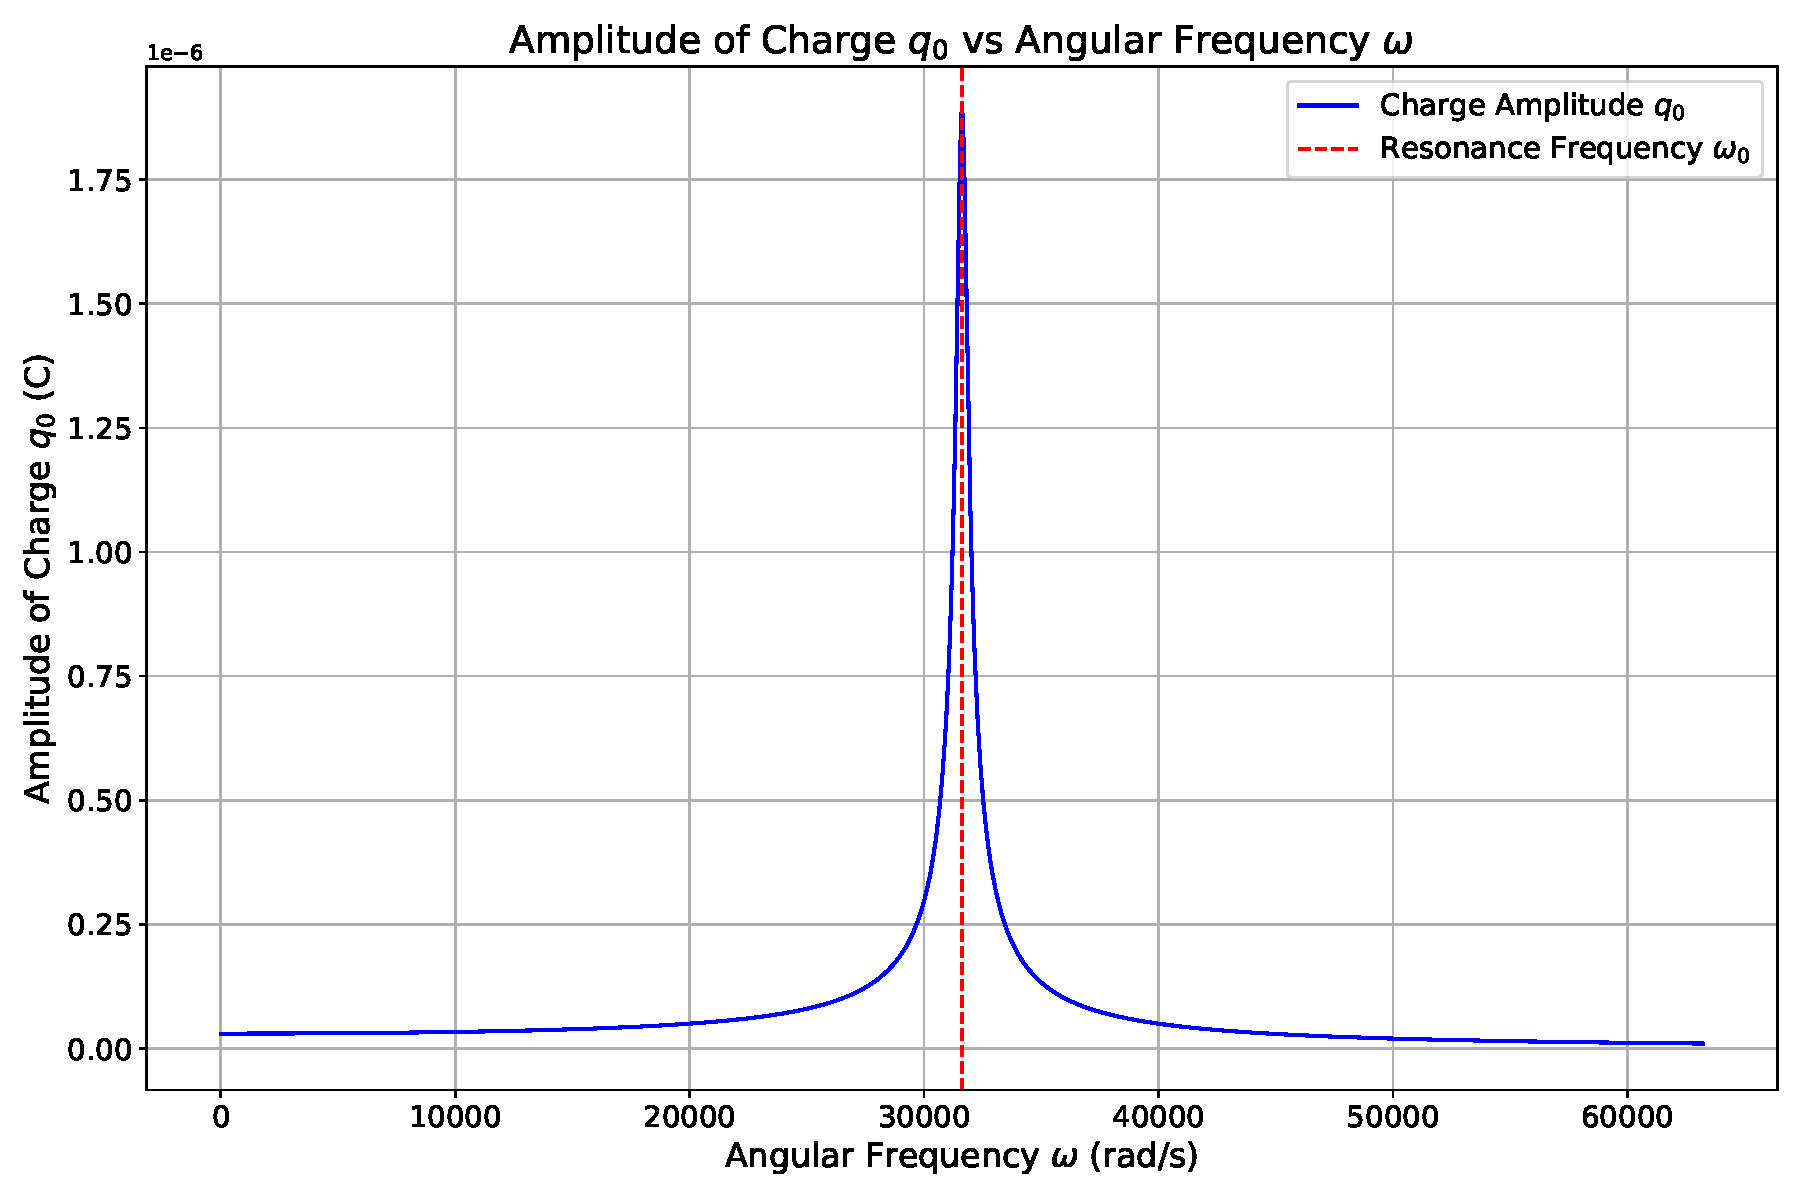
\includegraphics[width=1\linewidth]{figs/fig_sol_2.5f.pdf}
    %\caption{Caption}
   % \label{fig:enter-label}
\end{figure}
\\\textbf{Solution(g)}
\\
\\Voltage across a capacitor is maximum when the charge carried by it maximum. To find the value of $\omega$ for which $q_0$ is maximum, we differentiate $q_0$ with respect to $\omega$ and then equate it to zero.
\[\frac{dq_0}{d\omega}=\frac{V_0}{L}\frac{d}{d\omega}\left(\left[\left(\omega_0^2-\omega^2\right)^2+(\gamma\omega)^2\right]^{-1/2}\right)\]
\[=-\frac{1}{2}\left[\left(\omega_0^2-\omega^2\right)^2+(\gamma\omega)^2\right]^{-3/2}\times\left(2\left(\omega_0^2-\omega^2\right)\times-2\omega+2\omega\gamma^2\right)=0\]
\[\Rightarrow-2\left(\omega_0^2-\omega^2\right)\times2\omega+2\omega\gamma^2=0\Rightarrow2\left(\omega_0^2-\omega^2\right)=\gamma^2\]
\[\Rightarrow \omega=\sqrt{\frac{2\omega_0^2-\gamma^2}{2}}=\sqrt{\frac{1}{2}\left(\frac{2}{LC}-\left(\frac{R}{L}\right)^2\right)}=\sqrt{\frac{1}{2}\left(\frac{2}{0.1\times10^{-8}}-\left(\frac{50}{10^{-8}}\right)^2\right)}\approx3.162\times10^4\,\text{rad\,s}^{-1}.\]

\end{document}